%Version 3.1 December 2024 -- Springer Nature LaTeX template (sn-jnl), official package
%downloaded from resource-cms.springernature.com on 2026-10-23 (see report/final/README.md).
%Numbered Math and Physical Sciences reference style.
\documentclass[pdflatex,sn-mathphys-num,onecolumn]{sn-jnl}

\usepackage{graphicx}%
\usepackage{multirow}%
\usepackage{amsmath,amssymb,amsfonts}%
\usepackage{amsthm}%
\usepackage{mathrsfs}%
\usepackage[title]{appendix}%
\usepackage{xcolor}%
\usepackage{textcomp}%
\usepackage{manyfoot}%
\usepackage{booktabs}%
\usepackage{array}%
\usepackage{tabularx}%
\usepackage{xurl}%
\usepackage{tikz}%
\usepackage{stfloats}%
\usepackage{placeins}%
\usetikzlibrary{arrows.meta,positioning,fit,calc,backgrounds}%
\geometry{reset,paperwidth=210mm,paperheight=297mm,left=13.5mm,right=13.5mm,top=20mm,bottom=18mm,headheight=5.5pt,headsep=5.6mm,footskip=8mm,onecolumn}
\setlength\columnsep{6.3mm}
\setcounter{dbltopnumber}{3}
\renewcommand\dbltopfraction{0.9}
\renewcommand\dblfloatpagefraction{0.6}
\renewcommand\textfraction{0.05}
\renewcommand\topfraction{0.95}
\renewcommand\bottomfraction{0.9}
\renewcommand\floatpagefraction{0.85}
\setcounter{topnumber}{3}
\setcounter{bottomnumber}{2}
\setcounter{totalnumber}{5}
\makeatletter
\setlength\@fptop{0pt}
\setlength\@fpsep{18pt}
\setlength\@fpbot{0pt plus 1fil}
\makeatother
\newlength\origtw
\setlength\origtw{372pt}
\newenvironment{widefigure}[1][tbp]{\begin{figure*}[#1]\centering\begin{minipage}{\origtw}\setlength\textwidth{\origtw}\setlength\columnwidth{\origtw}}{\end{minipage}\end{figure*}}
\newenvironment{widetable}[1][tbp]{\begin{table*}[#1]\centering\begin{minipage}{\origtw}\setlength\textwidth{\origtw}\setlength\columnwidth{\origtw}\begin{center}\begin{threeparttable}\tablebodyfont\renewcommand\footnotetext[2][]{{\removelastskip\vskip3pt\let\tablebodyfont\tablefootnotefont\hskip0pt\if!##1!\else{\smash{$^{##1}$}}\fi##2\par}}}{\end{threeparttable}\end{center}\end{minipage}\end{table*}}


\theoremstyle{thmstyleone}%
\newtheorem{theorem}{Theorem}%

\raggedbottom
\emergencystretch=3em
\sloppy

% Values from the audit runs (see report/final/evidence_ledger.md).
\newcommand{\LATMS}{20.9\,ms}
\newcommand{\LATIQR}{20.2--21.9\,ms}

% ---------------------------------------------------------------------------
% Evidence links. Every code and result link is pinned to the audited commit.
% \ev{path#anchor}{shown text}: the shown text is typeset as a breakable URL.
% ---------------------------------------------------------------------------
\newcommand{\repo}{https://github.com/not-good-keeper/compact-vit-sign-language/blob/3330b87d607eac34615517c092f79fc3e3abf1b6}
\newcommand{\treeurl}{https://github.com/not-good-keeper/compact-vit-sign-language/tree/3330b87d607eac34615517c092f79fc3e3abf1b6}
\newcommand{\ev}[2]{\href{\repo/#1}{\nolinkurl{#2}}}
\newcommand{\evdir}[2]{\href{\treeurl/#1}{\nolinkurl{#2}}}
\newcommand{\new}[1]{\nolinkurl{#1}}
% Source note under a figure: one short paragraph, same style as a table footnote.
\newcommand{\src}[1]{\par\vspace{3pt}{\footnotesize\raggedright\setlength{\parindent}{0pt}#1\par}}
\newcolumntype{L}[1]{>{\raggedright\arraybackslash\hspace{0pt}}p{#1}}
\newcolumntype{Y}{>{\raggedright\arraybackslash\hspace{0pt}}X}

\definecolor{cA}{HTML}{2a78d6}
\definecolor{cB}{HTML}{eb6834}
\definecolor{cC}{HTML}{1baf7a}
\definecolor{cD}{HTML}{eda100}
\definecolor{ink2}{HTML}{52514e}
\definecolor{panel}{HTML}{f3f2ef}
\tikzset{
  box/.style={draw=ink2, rounded corners=2pt, align=center, font=\footnotesize, inner sep=3pt, minimum height=7mm, fill=white},
  stage/.style={box, fill=panel},
  arr/.style={-{Stealth[length=2.2mm]}, draw=ink2, line width=0.6pt},
  lab/.style={font=\scriptsize, text=ink2, align=center},
}


\usepackage{xr-hyper}
\externaldocument{main}
\renewcommand{\thefigure}{S\arabic{figure}}
\renewcommand{\thetable}{S\arabic{table}}
\renewcommand{\thesection}{S\arabic{section}}

\begin{document}

\title[Compact factorised ViT for isolated ISL words]{Supplementary Information for ``ISL-ViT-Tiny: A Compact Factorised Vision Transformer for Isolated-Word Indian Sign Language Recognition, Evaluated on Held-Out Recording Sessions''}

\author[1]{\fnm{Nethi} \sur{Kushala Kumar}}
\author[1]{\fnm{Yalamanchi} \sur{Kushal}}
\author[1]{\fnm{Bagyammal} \sur{Thirumurthy}}
\author[1]{\fnm{Dhruseek} \sur{Rishi Menon}}

\affil[1]{\orgdiv{Department of Computer Science and Engineering}, \orgname{Amrita School of Computing, Amrita Vishwa Vidyapeetham}, \orgaddress{\city{Coimbatore}, \country{India}}}

\maketitle

\section{Supplementary figures and tables}\label{supp:items}
Each supplementary figure and table extends a section of the main text, as follows.
\begin{itemize}\setlength{\itemsep}{1pt}\setlength{\parskip}{0pt}
\item \textit{Closest prior work.} Supplementary Table~\ref{tab:lit} places the closest works beside this project; numbers are as reported by each paper (main text, Section~\ref{sec:related}).
\item \textit{Data and region extraction.} Supplementary Fig.~\ref{fig:exdata} shows frames from INCLUDE and CISLR, and Supplementary Fig.~\ref{fig:excrops} shows the hand and face crops that region extraction produces (Sections~\ref{sec:method:data} and~\ref{sec:method:pre}).
\item \textit{Model overview.} Supplementary Fig.~\ref{fig:model} summarises the network of Section~\ref{sec:method:model} in one diagram; Fig.~\ref{fig:archmodel} of the main text gives the detailed architecture.
\item \textit{Experimental setup.} Supplementary Table~\ref{tab:setup} lists, for each principal experiment, the models compared, the test set, the number of seeds and the metric (Section~\ref{sec:setup}).
\item \textit{Additional results.} Supplementary Figs.~\ref{fig:variants} to~\ref{fig:perclass} show the variant comparison, the temporal-length and crop-size ablations, and per-word recall (Sections~\ref{sec:res:variants}, \ref{sec:res:ablation} and~\ref{sec:res:perclass}).
\item \textit{Super-resolution study.} Supplementary Fig.~\ref{fig:gan} shows the design of the study, Supplementary Figs.~\ref{fig:exgan} and~\ref{fig:exdetect} show what each front end does to a 180p clip, and Supplementary Table~\ref{tab:gan} gives the results of every arm (Sections~\ref{sec:method:sr} and~\ref{sec:res:gan}).
\item \textit{Claimed contributions.} Supplementary Table~\ref{tab:contrib} ties each claim of Section~\ref{sec:discussion} to its evidence.
\end{itemize}

\begin{table*}[!htbp]
\caption{Closest prior work. Results are as reported by each source.}\label{tab:lit}
\scriptsize
\setlength{\tabcolsep}{2.5pt}
\begin{tabularx}{\textwidth}{@{}L{2.5cm}L{3.3cm}L{3.6cm}YL{3.3cm}@{}}
\toprule
Work & Data and task & Model and input & Protocol and reported result & Relation to this project \\
\midrule
INCLUDE~\cite{sridhar2020include} & ISL, 263 and 50 words & pretrained extractor and encoder, trained decoder; RGB video & dataset split; 85.6\% (263), 94.5\% (50) & same corpus; we hold out sessions \\\addlinespace[2.5pt]
OpenHands~\cite{selvaraj2022openhands} & 6 sign languages incl.\ INCLUDE & LSTM, BERT, ST-GCN, SL-GCN; pose keypoints & INCLUDE: 93.5\% (SL-GCN), 94.7\% with pretraining & keypoints only; dataset split \\\addlinespace[2.5pt]
CISLR~\cite{joshi2022cislr} & ISL, about 4,700 words & prototype one-shot; I3D features & 16.81\% top-1 (v1.0-a) & our cross-corpus test set \\\addlinespace[2.5pt]
SPOTER~\cite{bohacek2022spoter} & American WLASL, Argentinian LSA64 & Transformer; 2D pose & WLASL100 63.18\%; LSA64 100\% & normalised hand pose, as in our features \\\addlinespace[2.5pt]
SAM-SLR~\cite{jiang2021samslr} & Turkish AUTSL & GCN and CNN ensemble; skeleton, RGB, depth & signer-independent challenge; 98.42\% (RGB track) & multimodal fusion; much larger \\\addlinespace[2.5pt]
AUTSL~\cite{sincan2020autsl} & Turkish, 226 signs & CNN and LSTM; RGB and depth & 95.95\% random vs 62.02\% user-independent & split changes the conclusion \\\addlinespace[2.5pt]
Tiny\-MSLR~\cite{lamaakal2026tinymslr} & 20 classes from German PHOENIX-2014T and Chinese Sign Language (CSL) & ConvNeXt-Tiny and Swin, distilled; RGB & signer-independent; 99.01\% validation; under 2.7\,M parameters, 7.2\,MB & edge target; smaller task \\\addlinespace[2.5pt]
Kannada study~\cite{venkatappa2026kannada} & Kannada Sign Language, 33 words & LSTM, bidirectional LSTM, Transformer; MediaPipe landmarks & 94.19 to 95.71\%; 1,098\,KB on phone & phone deployment \\\addlinespace[2.5pt]
Nedungadi et al.~\cite{nedungadi2025vit} & ISL, domain dataset & CNN and ViT; RGB & 97.5\% under optimised conditions & ISL system; protocol differs \\
\midrule
This work & ISL INCLUDE, 262 trained, 50 deployed & factorised ViT, 4-bit; 3 crops and hand landmarks & held-out sessions; 85.9\% masked-50, 3 seeds; 2,069,700\,B & -- \\
\botrule
\end{tabularx}
\end{table*}

\begin{figure*}[!htbp]
\centering
\includegraphics[width=\textwidth]{figures/fig_ex_dataset.png}
\caption{Examples from the corpora. (a)~INCLUDE~\cite{sridhar2020include}: the middle frame of one training clip from each of ten of its fifteen word categories. Every clip is 1920$\times$1080 and shows one signer standing in front of a wall. (b)~Eight frames, evenly spaced from 5\% to 95\% of one clip of ``Thank you''. (c)~Six CISLR~\cite{joshi2022cislr} clips, used only as the cross-corpus test: they are 300 pixels across and show other signers, backgrounds and cameras. Frames from the iSign~\cite{joshi2024isign} clips used for unlabelled pretraining are not shown.}\label{fig:exdata}
\end{figure*}

\begin{figure*}[!htbp]
\centering
\includegraphics[width=\textwidth]{figures/fig_ex_crops.png}
\caption{Region extraction on training clips. (a)~One clip (``they''). Each letterboxed frame carries the left-hand, right-hand and face boxes (blue, orange, green), and the three crops under it are the 128-pixel images stored in the cache; the model reads them at 64 pixels. The columns are every fourth of the 32 stored frames, and the model uses 16 of the 32. (b)~The three crops at frame 17 of four other words. (c)~Crops grouped by how their box was obtained. \emph{Direct}: from the holistic landmarks. \emph{Forearm region rescue}: the dedicated hand detector found the hand inside the region predicted from the body pose. \emph{Interpolated}: no detector fired on that frame, so the nearest real box was reused and the frame is flagged. \emph{No box}: the detectors fired on no frame of the clip, and the crop is a zero tensor.}\label{fig:excrops}
\end{figure*}

\begin{widefigure}[!htbp]
\centering
\resizebox{\linewidth}{!}{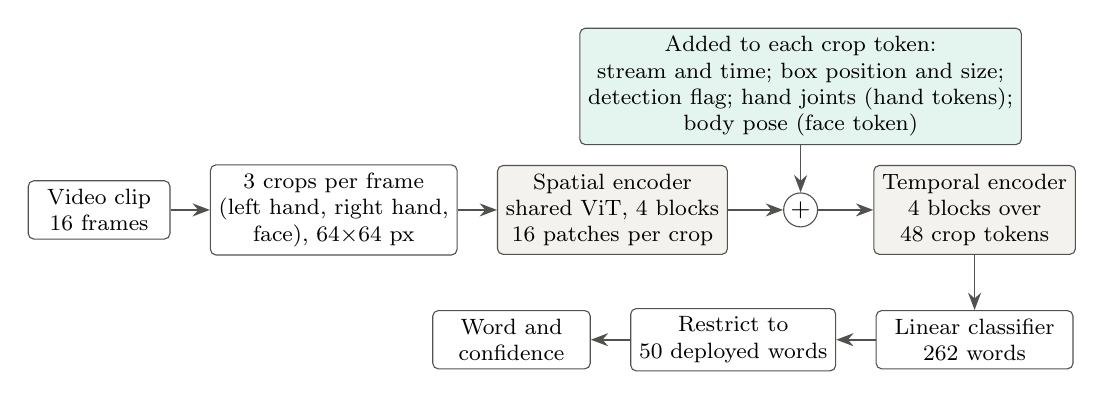
\begin{tikzpicture}[node distance=5mm and 5mm]
\node[box, minimum width=18mm] (in) {Video clip\\16 frames};
\node[box, right=of in, minimum width=27mm] (crops) {3 crops per frame\\(left hand, right hand,\\face), $64{\times}64$ px};
\node[stage, right=of crops, minimum width=25mm] (spat) {Spatial encoder\\shared ViT, 4 blocks\\16 patches per crop};
\node[circle, draw=ink2, inner sep=1pt, font=\small, right=7mm of spat] (plus) {$+$};
\node[box, above=6mm of plus, minimum width=44mm, fill=cC!12] (cond) {Added to each crop token:\\stream and time; box position and size;\\detection flag; hand joints (hand tokens);\\body pose (face token)};
\node[stage, right=7mm of plus, minimum width=25mm] (temp) {Temporal encoder\\4 blocks over\\48 crop tokens};
\node[box, below=7mm of temp, minimum width=25mm] (head) {Linear classifier\\262 words};
\node[box, left=of head, minimum width=25mm] (mask) {Restrict to\\50 deployed words};
\node[box, left=of mask, minimum width=20mm] (out) {Word and\\confidence};
\draw[arr] (in) -- (crops);
\draw[arr] (crops) -- (spat);
\draw[arr] (spat) -- (plus);
\draw[arr] (cond) -- (plus);
\draw[arr] (plus) -- (temp);
\draw[arr] (temp) -- (head);
\draw[arr] (head) -- (mask);
\draw[arr] (mask) -- (out);
\end{tikzpicture}}
\caption{ISL-ViT-Tiny. Attention is factorised: first within each crop, then across the 48 crop tokens of the clip. Shaded boxes are Transformer stacks; the green box holds the additive token-conditioning terms of Eq.~\eqref{eq:token}.}\label{fig:model}
\src{Source: \ev{islvit/models/isl_vit.py\#L136-L299}{isl_vit.py:136-299} (model), \ev{islvit/models/isl_vit.py\#L312-L344}{isl_vit.py:312-344} (landmark features), \ev{islvit/mask50.py\#L56-L108}{mask50.py:56-108} (50-word restriction). Parameter counts from \new{report/final/scripts/measure_model.py}.}
\end{widefigure}

\begin{widetable}[!htbp]
\caption{Settings of the principal experiments.}\label{tab:setup}
\scriptsize
\setlength{\tabcolsep}{3pt}
\begin{tabularx}{\textwidth}{@{}L{2.3cm}YL{2.6cm}L{1.4cm}L{2.0cm}@{}}
\toprule
Experiment & Models compared & Test set & Seeds & Metric \\
\midrule
Main result and variants & pixel FP32; landmark FP32; landmark PTQ INT4; landmark QAT INT4 (released) & 472 clips, 50 words, held-out sessions & 3 each & masked-50, 6-view TTA \\\addlinespace[2.5pt]
Protocol comparison & one 50-word pixel recipe on random-video and session-disjoint splits & 200 and 472 clips (each protocol's own test set) & 1 and 2 & top-1, single view \\\addlinespace[2.5pt]
Official split & released recipe (landmark FP32, then QAT INT4) trained on INCLUDE's own training clips & 191 clips (INCLUDE-50) and 816 clips (262 words), official test sets & 1 & top-1, single view and TTA \\\addlinespace[2.5pt]
Temporal length & 8, 16, 24, 32 frames from one 32-frame cache, 50-word pixel recipe & 472 clips & 1 (16 frames: 2) & top-1, single view and TTA \\\addlinespace[2.5pt]
Crop resolution & 64, 112, 128 pixel input, early 8-frame recipe & INCLUDE-50 take-group, 159 clips & 1 & top-1 \\\addlinespace[2.5pt]
Cross-corpus & released models on CISLR & 609 CISLR clips & 3 & top-1 \\\addlinespace[2.5pt]
Super-resolution & bicubic, SR-L1, SR-GAN v1, v2, v3, v3 control; frozen INT4 classifiers & 472 clips degraded to 360p, 240p, 180p & 3 & masked-50, TTA; McNemar \\
\botrule
\end{tabularx}
\end{widetable}

\begin{widefigure}[!htbp]
\centering
\includegraphics[width=\textwidth]{figures/fig_variants.pdf}
\caption{Controlled variant comparison on the deployed test set. (a) Top-1 accuracy of each seed (markers) and the three-seed mean (bar). (b) For each seed, the test clips that the second model gets right and the first gets wrong (gained) or the reverse (lost), with the exact McNemar $p$ for that seed.}\label{fig:variants}
\src{Data: \ev{runs/f16_262w_s0/masked50_clean.json}{runs/f16_262w_s*/masked50_clean.json}, \ev{runs/f16_262w_lm_s0/masked50_clean.json}{runs/f16_262w_lm_s*/masked50_clean.json}, \ev{runs/f16_262w_lm_s0/ptq4_clean.json}{runs/f16_262w_lm_s*/ptq4_clean.json}, \ev{runs/f16_262w_lm_s0_qat4/masked50_clean.json}{runs/f16_262w_lm_s*_qat4/masked50_clean.json} (keys \texttt{masked\_tta.top1}, \texttt{hits\_masked\_tta}); training \ev{run_landmarks.sh}{run_landmarks.sh}, \ev{run_lm_qat.sh}{run_lm_qat.sh}; statistics and plot \new{report/final/scripts/audit_results.py}, \new{make_figures.py}.}
\end{widefigure}

\begin{widefigure}[!htbp]
\centering
\includegraphics[width=\textwidth]{figures/fig_ablation.pdf}
\caption{Temporal length and crop resolution. (a) Top-1 of the 50-word pixel-only recipe with 8, 16, 24 or 32 frames sampled from the same 32-frame cache, single view and six-view TTA; at 16 frames the line is the mean of two seeds (dots). (b) Top-1 at three crop sizes, early 8-frame recipe, INCLUDE-50 take-group split (159 clips, one seed).}\label{fig:ablation}
\src{Data: (a) \ev{runs/f8_clean_s0/summary.json}{runs/f8_clean_s0}, \ev{runs/f16_clean_s0/summary.json}{f16_clean_s0}, \ev{runs/f16_clean_s1/summary.json}{f16_clean_s1}, \ev{runs/f24_clean_s0/summary.json}{f24_clean_s0}, \ev{runs/f32_clean_s0/summary.json}{f32_clean_s0} (keys \texttt{test}, \texttt{test\_tta}); launch \ev{run_frames32.sh}{run_frames32.sh}. (b) \ev{runs/abl64__take-group/summary.json}{runs/abl64__take-group}, \ev{runs/abl112__take-group/summary.json}{abl112__take-group}, \ev{runs/abl128__take-group/summary.json}{abl128__take-group}; launch \ev{run_ablation_res.sh}{run_ablation_res.sh}.}
\end{widefigure}

\begin{widefigure}[!htbp]
\centering
\includegraphics[width=\textwidth]{figures/fig_perclass.pdf}
\caption{Per-word recall of the released model on the 472 test clips, pooled over the three released seeds (about 9 to 11 test clips per word per seed), sorted. Dotted lines mark 50\% and 90\%.}\label{fig:perclass}
\src{Data: \texttt{hits\_masked\_tta} and \texttt{video\_paths} in \ev{runs/f16_262w_lm_s0_qat4/masked50_clean.json}{runs/f16_262w_lm_s*_qat4/masked50_clean.json}; computed by \new{make_figures.py}.}
\end{widefigure}

\begin{widefigure}[!htbp]
\centering
\resizebox{\linewidth}{!}{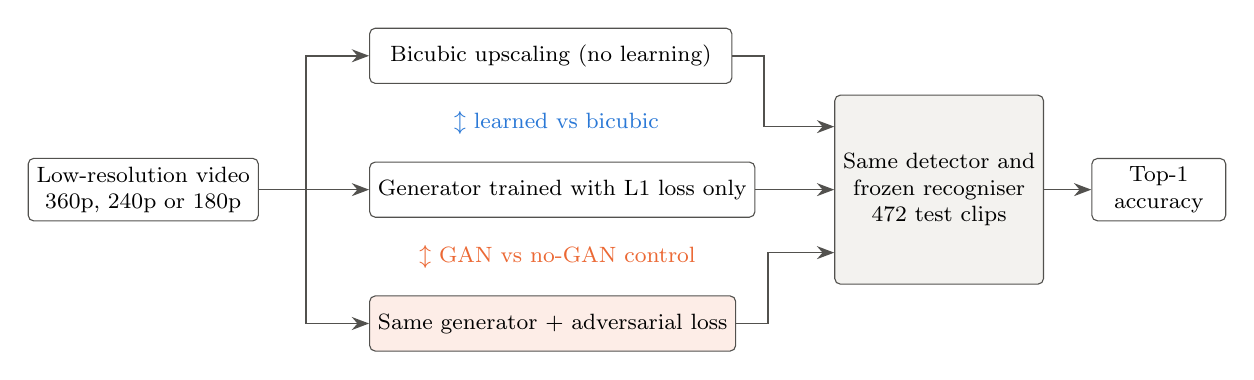
\begin{tikzpicture}[node distance=4mm and 6mm]
\node[box, minimum width=26mm] (lr) {Low-resolution video\\360p, 240p or 180p};
\node[box, right=14mm of lr, yshift=17mm, minimum width=46mm] (bic) {Bicubic upscaling (no learning)};
\node[box, right=14mm of lr, minimum width=46mm] (l1) {Generator trained with L1 loss only};
\node[box, right=14mm of lr, yshift=-17mm, minimum width=46mm, fill=cB!12] (gan) {Same generator + adversarial loss};
\node[font=\footnotesize, text=cA] at ($(bic.south)!0.5!(l1.north)$) {$\updownarrow$ learned vs bicubic};
\node[font=\footnotesize, text=cB] at ($(l1.south)!0.5!(gan.north)$) {$\updownarrow$ GAN vs no-GAN control};
\node[stage, right=10mm of l1, minimum width=26mm, minimum height=24mm] (rec) {Same detector and\\frozen recogniser\\472 test clips};
\node[box, right=6mm of rec, minimum width=17mm] (acc) {Top-1\\accuracy};
\draw[arr] (lr.east) -- ++(6mm,0) |- (bic.west);
\draw[arr] (lr.east) -- (l1.west);
\draw[arr] (lr.east) -- ++(6mm,0) |- (gan.west);
\draw[arr] (bic.east) -- ++(4mm,0) |- ([yshift=8mm]rec.west);
\draw[arr] (l1.east) -- (rec.west);
\draw[arr] (gan.east) -- ++(4mm,0) |- ([yshift=-8mm]rec.west);
\draw[arr] (rec) -- (acc);
\end{tikzpicture}}
\caption{Design of the super-resolution comparison. Only the upscaling step changes between arms: bicubic versus a learned upscaler measures what learning to upscale buys, and a GAN versus the same generator without its discriminator measures what the adversarial term buys. v3 has its own matched control.}\label{fig:gan}
\src{Source: \ev{islvit/sr/models.py}{sr/models.py} (networks), \ev{islvit/sr/train.py\#L137-L382}{sr/train.py:137} (training), \ev{islvit/data/crops.py\#L163-L204}{crops.py:163} (insertion point); drivers \ev{run_gan_study.sh}{run_gan_study.sh}, \ev{run_gan_v3.sh}{run_gan_v3.sh}. Generator SHA-256 hashes are recorded in \evdir{runs/gan_study/detection}{runs/gan_study/detection/*.json}.}
\end{widefigure}

\begin{figure*}[!htbp]
\centering
\includegraphics[width=\textwidth]{figures/fig_ex_gan.png}
\caption{What each front end does to the hand region of a 180p clip. For three test clips drawn at random, the hand box that the detector finds in the middle frame of the 1080p clip (first column) is cut from the frame the detector would see after each front end. The second column is the 180p, JPEG-quality-40 input enlarged by nearest neighbour; the other columns are the 720p result of bicubic interpolation, the generator trained with L1 loss only, and the GAN generators v2 and v3. PSNR is measured on the crop against the 1080p source; the figures over 1,200 held-out patches are in Table~\ref{tab:gan}.}\label{fig:exgan}
\end{figure*}

\begin{widetable}[!htbp]
\caption{Super-resolution study at 180p (frozen INT4 models, 472 clips, three seeds). Detection is the share of frames with a genuine left-hand detection; on the clean test cache it is 92.0\%. Image quality, as PSNR and structural similarity index measure (SSIM), is measured on 1,200 held-out patches.}\label{tab:gan}
\footnotesize
\setlength{\tabcolsep}{4pt}
\begin{tabular*}{\textwidth}{@{\extracolsep\fill}lccccc@{}}
\toprule
Front end & GAN loss & Top-1 (\%) & Left hand found (\%) & PSNR (dB) & SSIM \\
\midrule
Bicubic & -- & 61.0 & 51.0 & 30.07 & 0.856 \\
SR-L1 & no & 76.0 & 68.2 & 31.83 & 0.900 \\
SR-GAN v1 & yes & 75.4 & 67.9 & 31.07 & 0.883 \\
SR-GAN v2 & yes & 75.5 & 68.6 & 31.09 & 0.884 \\
v3 without GAN & no & 75.6 & 65.5 & 29.96 & 0.863 \\
SR-GAN v3 & yes & 75.4 & 77.6 & 29.76 & 0.870 \\
\botrule
\end{tabular*}
\src{Sources: \new{runs/gan_study/frozen_int4/L3_*.json} and \new{runs/gan_study_v1/frozen_int4/L3_*.json}; \new{runs/gan_study/detection/L3_*.json} and \new{runs/gan_study_v1/detection/L3_srgan.json} (\texttt{streams.left\_hand.genuine}); \new{runs/gan_study/sr_quality*.json} and \new{runs/gan_study_v1/sr_quality.json} (level \texttt{L3 180p}).}
\end{widetable}

\begin{figure*}[!htbp]
\centering
\includegraphics[width=\textwidth]{figures/fig_ex_detect.png}
\caption{Landmark detection after each front end on one 180p frame. Each row is a frame from a test clip, shown in a window around the signer, with the box and 21 joints of every hand the detector returned; blue marks the left hand and orange the right. A hand counts as \emph{found} when its box overlaps the box found on the 1080p frame (intersection over union of at least 0.3), as \emph{misplaced} when a box is returned elsewhere, and as \emph{missed} when none is returned. The frames came from 36 test clips taken in random order: rows 1 and 2 are frames where every learned front end found more hands than bicubic, and row 3 is a frame where all four front ends found both. They were chosen to show the mechanism and say nothing about rates, which are in Table~\ref{tab:gan}.}\label{fig:exdetect}
\end{figure*}

\begin{widetable}[!htbp]
\caption{Claimed contributions, closest prior approach and evidence.}\label{tab:contrib}
\scriptsize
\setlength{\tabcolsep}{3pt}
\begin{tabularx}{\textwidth}{@{}L{3.0cm}L{3.6cm}Y@{}}
\toprule
Contribution & Closest prior approach & Evidence in this project \\
\midrule
Crops and landmarks in one token stream & pose-only models~\cite{selvaraj2022openhands,bohacek2022spoter}; multimodal ensembles~\cite{jiang2021samslr} & +12.8 points over pixels only, 3 seeds, paired $p\le5\times10^{-9}$ per seed (Fig.~\ref{fig:variants}) \\\addlinespace[2.5pt]
2\,MB 4-bit model & QAT~\cite{jacob2018quant}; group scales~\cite{shen2020qbert,frantar2023gptq} & 2,069,700\,B; PTQ 83.4\% vs QAT 85.9\%, pooled $p=0.0012$; QAT level with FP32 (pooled $p=0.44$) \\\addlinespace[2.5pt]
Session-aware evaluation & user-independent benchmark split~\cite{sincan2020autsl} & 13 blocks, none crossing train/test; 98.5\% vs 70.1\% for one recipe \\\addlinespace[2.5pt]
GAN with a no-GAN control & task-driven SR~\cite{haris2018taskdriven}; SR for vision tasks~\cite{dai2016srhelpful} & learned SR +14 to +15 points at 180p; adversarial term +1.5 to +2.4 at 240p \\
\botrule
\end{tabularx}
\end{widetable}


\section{Experiment traceability}\label{app:trace}

Table~\ref{tab:trace} lists, for each experiment reported in this paper, the question it answers and the single change it controls, the launch script, the raw result files, and the table, figure or section where the result appears. Every link is pinned to the audited commit, so each number can be traced to the file it was read from.

\begin{table*}[!htbp]
\caption{Experiment traceability. Links are pinned to commit \texttt{3330b87}.}\label{tab:trace}
\scriptsize
\setlength{\tabcolsep}{2.5pt}
\begin{tabularx}{\textwidth}{@{}L{0.7cm}L{3.6cm}L{4.1cm}YL{1.7cm}@{}}
\toprule
ID & Question; controlled change & Launch & Raw result & Shown in \\
\midrule
E1 & Landmark gain; landmark stream on or off & \ev{run_landmarks.sh}{run_landmarks.sh} & \ev{runs/f16_262w_s0/masked50_clean.json}{f16_262w_s*/masked50_clean.json}, \ev{runs/f16_262w_lm_s0/masked50_clean.json}{f16_262w_lm_s*/masked50_clean.json} & Tab.~\ref{tab:variants}, Fig.~\ref{fig:variants} \\\addlinespace[2.5pt]
E2 & 4-bit cost; PTQ or QAT & \ev{run_lm_qat.sh}{run_lm_qat.sh} & \ev{runs/f16_262w_lm_s0/ptq4_clean.json}{f16_262w_lm_s*/ptq4_clean.json}, \ev{runs/f16_262w_lm_s0_qat4/masked50_clean.json}{f16_262w_lm_s*_qat4/masked50_clean.json} & Tab.~\ref{tab:variants} \\\addlinespace[2.5pt]
E3 & Clean test cache; fresh detector per video & \ev{run_clean_test.sh}{run_clean_test.sh} & \ev{runs/f16_262w_lm_s0/masked50_fresh.json}{masked50_fresh.json} vs \texttt{\_clean} & Sec.~\ref{sec:method:pre} \\\addlinespace[2.5pt]
E4 & Leakage size; split protocol & \ev{run_frames32.sh}{run_frames32.sh} & \ev{runs/baseline_random_s0/summary.json}{baseline_random_s0}, \ev{runs/f16_clean_s0/summary.json}{f16_clean_s0}, \ev{runs/f16_clean_s1/summary.json}{f16_clean_s1} & Fig.~\ref{fig:protocol}a \\\addlinespace[2.5pt]
E5 & Protocol ladder; split protocol & \ev{run_phase2.sh}{run_phase2.sh} & \ev{runs/full263_v2__random-video/summary.json}{full263_v2__random-video}, \ev{runs/full263_v2__take-group/summary.json}{full263_v2__take-group}, \ev{runs/sd_full263/summary.json}{sd_full263} & Fig.~\ref{fig:protocol}b \\\addlinespace[2.5pt]
E6 & Checkpoint choice, folding; last vs best-val, validation folded & \ev{run_iter3.sh}{run_iter3.sh} & \ev{runs/sd263_lastsel/summary.json}{sd263_lastsel}, \ev{runs/sd263_foldval/summary.json}{sd263_foldval} & Sec.~\ref{sec:method:train} \\\addlinespace[2.5pt]
E7 & Seed noise; seed only (5 seeds) & \ev{run_lever2.sh}{run_lever2.sh} & \ev{runs/sd263_ssl_foldval/summary.json}{sd263_ssl_foldval}, \texttt{\_s1} to \texttt{\_s4} & Sec.~\ref{sec:method:metrics} \\\addlinespace[2.5pt]
E8 & Temporal length; frames drawn & \ev{run_frames32.sh}{run_frames32.sh} & \ev{runs/f8_clean_s0/summary.json}{f8_clean_s0}, \ev{runs/f24_clean_s0/summary.json}{f24_clean_s0}, \ev{runs/f32_clean_s0/summary.json}{f32_clean_s0} & Fig.~\ref{fig:ablation}a \\\addlinespace[2.5pt]
E9 & Crop size; input pixels & \ev{run_ablation_res.sh}{run_ablation_res.sh} & \ev{runs/abl64__take-group/summary.json}{abl64__take-group}, \ev{runs/abl112__take-group/summary.json}{abl112__take-group}, \ev{runs/abl128__take-group/summary.json}{abl128__take-group} & Fig.~\ref{fig:ablation}b \\\addlinespace[2.5pt]
E10 & Training length; epochs & \ev{run_longtrain.sh}{run_longtrain.sh}, \ev{run_push75.sh}{run_push75.sh} & \ev{runs/long2000_s1/summary.json}{long2000_s1}, \ev{runs/grok_wd005/summary.json}{grok_wd005}, \ev{runs/f16_long4k_s0/summary.json}{f16_long4k_s0} & Sec.~\ref{sec:res:ablation} \\\addlinespace[2.5pt]
E11 & Super-resolution; front end & \ev{run_gan_study.sh}{run_gan_study.sh}, \ev{run_gan_v3_test.sh}{run_gan_v3_test.sh} & \evdir{runs/gan_study}{runs/gan_study/}, \evdir{runs/gan_study_v1}{runs/gan_study_v1/} & Fig.~\ref{fig:ganres}, Tab.~\ref{tab:gan} \\\addlinespace[2.5pt]
E12 & Released model on CISLR; corpus & \new{run_crosscorpus_release.sh}$^{*}$ & \new{report/final/data/crosscorpus_release_s*.json}$^{*}$ & Sec.~\ref{sec:res:cross} \\\addlinespace[2.5pt]
E13 & Published benchmark; INCLUDE's own split & \new{run_official.sh}$^{*}$ & \new{runs/official_include50_lm_s0/official_eval.json}$^{*}$, \new{runs/official_include50_lm_s0_qat4/official_eval.json}$^{*}$, \new{runs/official_full263_lm_s0/official_eval.json}$^{*}$, \new{runs/official_full263_lm_s0_qat4/official_eval.json}$^{*}$; \new{report/final/data/official_split.json}$^{*}$ & Tab.~\ref{tab:sota} \\
\botrule
\end{tabularx}
\src{$^{*}$New in this report (\texttt{report/final/}). Evaluator for E1 to E3, E11 and E13: \ev{islvit/mask50.py\#L56-L108}{mask50.py}; for E4 to E10: \ev{islvit/train.py\#L244-L730}{train.py}, which scores the test split at the end of training.}
\end{table*}


\section{Architecture design and model iterations}\label{app:design}

Every number below comes from the main text or from the run file linked beside it; this section adds no new measurement.

\subsection{What the architecture borrows}

ISL-ViT-Tiny is assembled from four published designs; Table~\ref{tab:borrow} lists what each contributes and what was changed. The largest borrowing is the \emph{factorised encoder} of ViViT~\cite{arnab2021vivit}. ViViT describes four ways to apply a Transformer to video. Its Model~1 attends jointly over every space--time token; Model~2, the factorised encoder, runs a spatial Transformer on the tokens of each frame, reads out one [CLS] embedding per frame, and passes the sequence of frame embeddings to a temporal Transformer; Models~3 and~4 factorise attention inside each block instead. TimeSformer's divided space--time attention~\cite{bertasius2021timesformer} works like Model~3, alternating temporal and spatial attention within every block. ISL-ViT-Tiny follows Model~2 because no attention layer in it ever spans all the patches of a clip: the spatial stage attends within one image, and the temporal stage sees one token per image.

The change from ViViT is the unit that the spatial stage encodes. ViViT encodes a whole frame; ISL-ViT-Tiny encodes a detected crop, three per frame, so Stage~B receives $T\cdot S=48$ tokens rather than $T=16$ and needs a stream embedding to tell the left hand, the right hand and the face apart. Stage~B therefore attends across time and across body parts in one sequence, so it can relate the two hands to each other and to the face at any pair of frames. The attention cost of this arrangement can be counted directly. Per head and per layer, Stage~A computes $48\times17^2=13{,}872$ attention scores and Stage~B $49^2=2{,}401$, a total of 16,273. Joint attention over the 816 patch tokens of the clip would compute $816^2=665{,}856$, about 41 times as many.

Inside each stage the building blocks are those of ViT~\cite{dosovitskiy2021vit}: a strided convolution as patch embedding, a learned [CLS] token, a learned position embedding and pre-norm Transformer blocks. The dimensions are those of DeiT-Tiny~\cite{touvron2021deit} (width 192, three heads, MLP width 768), chosen so that ImageNet weights load into Stage~A without a projection layer. The loader copies the patch embedding, the [CLS] token and the first four of the twelve pretrained blocks, and resizes the $14\times14$ position grid to the $4\times4$ grid of a 64-pixel crop by bicubic interpolation (\ev{islvit/models/isl_vit.py\#L347-L377}{isl_vit.py:347}). The same width is what the iSign self-supervised checkpoint was trained at, which is why the model was never made narrower.

The self-supervised initialisation follows SimMIM~\cite{xie2022simmim} rather than the masked autoencoder (MAE) of He et al.~\cite{he2022mae}. The mask hides 75\% of the patches and is drawn jointly over time, stream and space, because a mask drawn inside each crop would let Stage~A solve the task alone and leave Stage~B untrained. MAE removes the masked tokens and encodes only the visible ones. With 16 patches per crop and a mask drawn over the whole clip, that would leave about four visible patches per crop, a different number in each crop. SimMIM instead replaces each masked patch with a learned mask token inside the encoder, so every crop keeps 17 tokens and the encoder that is pretrained is exactly the encoder that is later fine-tuned.

\begin{widetable}[!htbp]
\caption{Components taken from earlier ViTs and what ISL-ViT-Tiny changes.}\label{tab:borrow}
\scriptsize
\setlength{\tabcolsep}{3pt}
\begin{tabularx}{\textwidth}{@{}L{2.4cm}L{2.0cm}YY@{}}
\toprule
Component & Source & Kept & Changed \\
\midrule
Factorised encoder & ViViT Model~2~\cite{arnab2021vivit} & spatial Transformer per image, [CLS] readout, temporal Transformer over the readouts & the image is a hand or face crop, not a frame; 48 tokens per clip with stream embeddings \\\addlinespace[2.5pt]
Patch embedding, [CLS], position embedding, pre-norm block & ViT~\cite{dosovitskiy2021vit} & all, unchanged & 64-pixel input gives a $4\times4$ grid of 16 patches \\\addlinespace[2.5pt]
Width 192, 3 heads, MLP 768 & DeiT-Tiny~\cite{touvron2021deit} & dimensions and the first four pretrained blocks & four blocks per stage instead of twelve \\\addlinespace[2.5pt]
Masked image modelling & SimMIM~\cite{xie2022simmim} & learned mask token inside the encoder, pixel regression on masked patches & mask drawn across time, stream and space; crops without a real detection excluded from the loss \\\addlinespace[2.5pt]
Stochastic depth & Huang et al.~\cite{huang2016stochdepth} & drop rate rising to 0.1 with depth & -- \\\addlinespace[2.5pt]
Token conditioning & this work & -- & crop geometry, missing-detection flag, hand-landmark and body-pose vectors added to the crop tokens through zero-initialised MLPs \\
\botrule
\end{tabularx}
\end{widetable}

\subsection{What is added, and why}

Cropping removes two things a sign depends on: where the hand is, and its exact shape, which 64 pixels resolve only coarsely. The additions put both back without adding a single token. The box centre and size, a flag for crops that were interpolated rather than detected, a 65-number handshape and wrist-position vector per hand and a 21-number body-pose vector are each mapped to width 192 and added to the crop token they describe (Eq.~\eqref{eq:token}). The attention pattern, the sequence length and the temporal stage are therefore the same as in the pixel-only model. The last layer of every added MLP starts at zero, so at the first training step the network computes exactly what the pretrained pixel-only network computes. The side inputs then enter gradually, which is intended to keep early gradients from disturbing the transferred weights. The landmark features are computed inside the model from raw joint coordinates, so training and offline evaluation cannot compute them differently.

\subsection{How the model reaches 2\,MB}

The architecture fixes the parameter count at 3,894,214; quantisation sets the bytes. Stored in FP32, the weights take $3{,}894{,}214\times4=15{,}576{,}856$ bytes, about 15.6\,MB. For the 3.76\,M-parameter pixel-only model, 8-bit weights still took 3.70\,MB, nearly twice the budget (\ev{islvit/export.py\#L246-L262}{export.py:246}). Making the network smaller was the other route, and it was costly in a specific way: the width cannot fall below 192 without losing both the ImageNet and the self-supervised initialisations. A distillation student with two blocks per stage at width 192 was built for this purpose and measures 1.95\,MB packed (\ev{islvit/distill.py}{distill.py}). No training run of it is recorded: 4-bit weights met the budget with the full model first.

The 4-bit format stores every weight matrix in groups of 128 consecutive weights (Eq.~\eqref{eq:int4}). Each group keeps one FP16 scale, $\sigma_G=\max_{w\in G}|w|/7$, and 128 signed codes in $[-8,7]$, packed two per byte. One group therefore costs $128\times4+16=528$ bits, or 4.125 bits per weight, and the scales add 3.1\% to the codes. A single scale per matrix would be cheaper still, but the largest weight in a $768\times192$ matrix would then set the step size for all 147,456 weights and leave most of them on a few levels; a group of 128 confines each outlier's effect to its own group. Embeddings, LayerNorm parameters and biases stay in FP16. At 4.125 bits per weight the 3.89\,M parameters would need about 2.0\,MB. The released file, 2,069,700 bytes, also holds the FP16 tensors, the configuration and the word list. Relative to FP32 the file is 7.5 times smaller.

Rounding a trained FP32 model this way lowered masked-50 accuracy from 86.5\% to 83.4\% (\ev{runs/f16_262w_lm_s0/ptq4_clean.json}{ptq4_clean.json}). Quantisation-aware training recovers most of the loss. For 300 further epochs the forward pass uses the rounded weights and the gradient updates full-precision master weights through a straight-through estimator~\cite{bengio2013ste,jacob2018quant}; the released model scores 85.9\%, within seed noise of FP32. The scale is rounded to FP16 before the weights are reconstructed, and training and export call the same rounding functions, so the model that is scored is the file that is shipped (\ev{islvit/export.py\#L202-L238}{export.py:202}).

\subsection{Model iterations}

The FP32 model reached 86.5\% only after more than 80 recorded training and pretraining runs, spread over successive iterations of the network, its inputs and its training recipe, and only then was the landmark model quantised. Table~\ref{tab:iter} lists the steps that changed accuracy, in the order they were made. Three test sets were used along the way, so a comparison is valid only within a block of the table. Steps 1 to 4 were scored on all 262 words of the 1,010 held-out-session INCLUDE clips; steps 5 to 8 trained on the 50 deployed words only and were scored on the 472 test clips; steps 9 to 12 are the final protocol of Section~\ref{sec:method:metrics}.

\begin{widetable}[!htbp]
\caption{Model iterations in the order they were made. Each step keeps everything above it in the same block. Values are means over the seeds shown.}\label{tab:iter}
\scriptsize
\setlength{\tabcolsep}{3pt}
\begin{tabularx}{\textwidth}{@{}L{0.7cm}YL{1.0cm}L{0.8cm}L{3.5cm}@{}}
\toprule
Step & Change & Top-1 (\%) & Seeds & Run \\
\midrule
\multicolumn{5}{@{}l}{\textit{262 words, 1,010 test clips, single view}} \\
1 & Factorised crop ViT, 8 frames, ImageNet initialisation, best-validation checkpoint & 22.1 & 1 & \ev{runs/sd_full263/summary.json}{sd_full263} \\\addlinespace[2.5pt]
2 & Final weights kept; validation clips folded into training (1,957 to 2,845 clips) & 33.0 & 1 & \ev{runs/sd263_foldval/summary.json}{sd263_foldval} \\\addlinespace[2.5pt]
3 & Masked image modelling on CISLR; resolution jitter during fine-tuning & 39.9 & 2 & \ev{runs/sd263_ssl_rj_s0/summary.json}{sd263_ssl_rj_s*} \\\addlinespace[2.5pt]
4 & Masked image modelling on 17,896 iSign clips instead & 42.1 & 2 & \ev{runs/sd263_isign_rj_s0/summary.json}{sd263_isign_rj_s*} \\
\midrule
\multicolumn{5}{@{}l}{\textit{50 words, 472 test clips, single view}} \\
5 & Step 4 recipe on the 50-word tier, 250 epochs & 51.7 & 2 & \ev{runs/vocab50_s0/summary.json}{vocab50_s*} \\\addlinespace[2.5pt]
6 & 2,000 epochs & 59.6 & 2 & \ev{runs/long2000_s1/summary.json}{long2000_s1}, \ev{runs/grok_wd005/summary.json}{grok_wd005} \\\addlinespace[2.5pt]
7 & 16 frames instead of 8 & 66.1 & 2 & \ev{runs/cap_16f64/summary.json}{cap_16f64}, \ev{runs/cap_16f64_s1/summary.json}{cap_16f64_s1} \\\addlinespace[2.5pt]
8 & 16 frames drawn from a 32-frame cache; CISLR clips removed from training & 70.1 & 2 & \ev{runs/f16_clean_s0/summary.json}{f16_clean_s*} \\
\midrule
\multicolumn{5}{@{}l}{\textit{262 words trained, restricted to 50 at test, 472 test clips, six-view TTA}} \\
9 & Train on all 262 words, 1,000 epochs & 73.7 & 3 & \ev{runs/f16_262w_s0/masked50_clean.json}{f16_262w_s*} \\\addlinespace[2.5pt]
10 & Hand-landmark and body-pose inputs & 86.5 & 3 & \ev{runs/f16_262w_lm_s0/masked50_clean.json}{f16_262w_lm_s*} \\\addlinespace[2.5pt]
11 & 4-bit, rounded after training & 83.4 & 3 & \ev{runs/f16_262w_lm_s0/ptq4_clean.json}{ptq4_clean.json} \\\addlinespace[2.5pt]
12 & 4-bit, quantisation-aware training (released, 2,069,700 bytes) & 85.9 & 3 & \ev{runs/f16_262w_lm_s0_qat4/masked50_clean.json}{f16_262w_lm_s*_qat4} \\
\botrule
\end{tabularx}
\end{widetable}

Apart from the landmark inputs, the steps that mattered most were not architectural. Fixing checkpoint selection and folding validation into training (step 2) and training for longer (step 6) changed the recipe, not the network. Self-supervised initialisation helped once the input blur of the pretraining corpus was matched by resolution jitter (step 3). Doubling the frames from 8 to 16 (step 7) was the largest change to the model's input until landmarks. Step 8 changed two things at once, the 32-frame cache and the removal of CISLR clips from training, so its 4-point gain cannot be split between them; a cache with spare frames probably helps because the sampler can then jitter within each segment. Training on all 262 words and restricting the output to 50 at test time (step 9) scored 73.7\% against 72.7\% for the 50-word models of step 8 under the same six-view protocol, a difference within seed noise, and it keeps the other 212 words available. The hand landmarks (step 10) added 12.8 points for 91,008 parameters, more than every earlier change to resolution, capacity or schedule.

Several candidates were measured and dropped. A 96-pixel input lowered 16-frame accuracy from 66.1\% to 61.0\% (\ev{runs/cap_16f96/summary.json}{cap_16f96}, one seed). Pretraining natively on 16-frame clips reached a lower reconstruction loss but transferred worse, 60.0\% against 70.1\% (\ev{runs/f16_mim16_s0/summary.json}{f16_mim16_s0}). Fine-tuning the 262-word model on the 50-word softmax changed masked-50 TTA top-1 by $+2.8$, $-0.4$ and $-3.6$ points in the three seeds; two of the changes, in opposite directions, were significant by the exact McNemar test (20 clips gained against 7 lost, $p=0.019$; 11 against 28, $p=0.0095$) (\ev{runs/f16_262w_s0_narrow/summary.json}{f16_262w_s*_narrow}). Five further landmark variants, screened on validation clips with the test set untouched, gave no gain that held across seeds. The first two of these decisions rest on one seed each.

\bibliography{references}

\end{document}
